%%%%%%%%%%%%%%%%%%%%%%%%%%%%%%%%%%%%%%%%%
% Jacobs Landscape Poster
% LaTeX Template
% Version 1.1 (14/06/14)
%
% Created by:
% Computational Physics and Biophysics Group, Jacobs University
% https://teamwork.jacobs-university.de:8443/confluence/display/CoPandBiG/LaTeX+Poster
% 
% Further modified by:
% Nathaniel Johnston (nathaniel@njohnston.ca)
%
% This template has been downloaded from:
% http://www.LaTeXTemplates.com
%
% License:
% CC BY-NC-SA 3.0 (http://creativecommons.org/licenses/by-nc-sa/3.0/)
%
%%%%%%%%%%%%%%%%%%%%%%%%%%%%%%%%%%%%%%%%%

%----------------------------------------------------------------------------------------
%	PACKAGES AND OTHER DOCUMENT CONFIGURATIONS
%----------------------------------------------------------------------------------------

\documentclass[final]{beamer}

\usepackage[scale=1.24]{beamerposter} % Use the beamerposter package for laying out the poster

\usetheme{confposter} % Use the confposter theme supplied with this template

\setbeamercolor{block title}{fg=ngreen,bg=white} % Colors of the block titles
\setbeamercolor{block body}{fg=black,bg=white} % Colors of the body of blocks
\setbeamercolor{block alerted title}{fg=white,bg=dblue!70} % Colors of the highlighted block titles
\setbeamercolor{block alerted body}{fg=black,bg=dblue!10} % Colors of the body of highlighted blocks
% Many more colors are available for use in beamerthemeconfposter.sty

%-----------------------------------------------------------
% Define the column widths and overall poster size
% To set effective sepwid, onecolwid and twocolwid values, first choose how many columns you want and how much separation you want between columns
% In this template, the separation width chosen is 0.024 of the paper width and a 4-column layout
% onecolwid should therefore be (1-(# of columns+1)*sepwid)/# of columns e.g. (1-(4+1)*0.024)/4 = 0.22
% Set twocolwid to be (2*onecolwid)+sepwid = 0.464
% Set threecolwid to be (3*onecolwid)+2*sepwid = 0.708

\newlength{\sepwid}
\newlength{\onecolwid}
\newlength{\twocolwid}
\newlength{\threecolwid}
\setlength{\paperwidth}{48in} % A0 width: 46.8in
\setlength{\paperheight}{36in} % A0 height: 33.1in
\setlength{\sepwid}{0.024\paperwidth} % Separation width (white space) between columns
\setlength{\onecolwid}{0.22\paperwidth} % Width of one column
\setlength{\twocolwid}{0.464\paperwidth} % Width of two columns
\setlength{\threecolwid}{0.708\paperwidth} % Width of three columns
\setlength{\topmargin}{-0.5in} % Reduce the top margin size
%-----------------------------------------------------------

\usepackage{graphicx}  % Required for including images

\usepackage{booktabs} % Top and bottom rules for tables

\usepackage{amsmath}

%----------------------------------------------------------------------------------------
%	TITLE SECTION 
%----------------------------------------------------------------------------------------

\title{Computer model calibration as a method for design, with an application to wind turbine blades} % Poster title

\author{Carl Ehrett} % Author(s)

\institute{Clemson University Department of Mathematical Sciences} % Institution(s)

%----------------------------------------------------------------------------------------

\begin{document}

\addtobeamertemplate{block end}{}{\vspace*{2ex}} % White space under blocks
\addtobeamertemplate{block alerted end}{}{\vspace*{2ex}} % White space under highlighted (alert) blocks

\setlength{\belowcaptionskip}{2ex} % White space under figures
\setlength\belowdisplayshortskip{2ex} % White space under equations

\begin{frame}[t] % The whole poster is enclosed in one beamer frame

\begin{columns}[t] % The whole poster consists of three major columns, the second of which is split into two columns twice - the [t] option aligns each column's content to the top

\begin{column}{\sepwid}\end{column} % Empty spacer column

\begin{column}{\onecolwid} % The first column

%----------------------------------------------------------------------------------------
%	OBJECTIVES
%----------------------------------------------------------------------------------------

\begin{block}{Computer experiments}

Researchers increasingly look to computer experiments as a method for investigating phenomena for which it is difficult or impossible to acquire data through direct physical experimentation.

\end{block}

%----------------------------------------------------------------------------------------
%	INTRODUCTION
%----------------------------------------------------------------------------------------

\begin{block}{Computer model calibration}

Often computer models contain unknown inputs, called calibration inputs, the values of which must be estimated for successful simulation. Examples might include when a model's output depends upon a physical constant the value of which is unknown. 
The value of a calibration input is often estimated by combining observations of the simulator output with real-world experimental data. Previous explorations of computer model calibration have approached calibration as a matter of bringing a computer model into agreement with physical reality.

\end{block}

%------------------------------------------------

%\begin{alertblock}{Central idea}
%\begin{itemize}
%\item Previous explorations of computer model calibration have approached calibration as a matter of bringing a computer model into agreement with physical reality.
%
%\item In the present work, we consider computer model calibration as a method for design. 
%
%\item Under this framework, we calibrate a computer model not using physical experimental data, but rather using ``desired data'' which describes the performance one hopes to achieve in the simulated system. 
%
%\end{itemize}
%
%\end{alertblock} 

%----------------------------------------------------------------------------------------

\end{column} % End of the first column

\begin{column}{\sepwid}\end{column} % Empty spacer column

\begin{column}{\twocolwid} % Begin a column which is two columns wide (column 2)

\begin{columns}[t,totalwidth=\twocolwid] % Split up the two columns wide column

\begin{column}{\onecolwid}\vspace{-.6in} % The first column within column 2 (column 2.1)

%----------------------------------------------------------------------------------------
%	MATERIALS
%----------------------------------------------------------------------------------------

\begin{block}{Gaussian process emulator}

Gaussian processes (GPs) can be thought of as generalizations of multivariate normal random variables. Whereas a multivariate normal random variable is a random vector of finite length, a GP is a random function. Just as a multivariate random variable is characterized by its mean vector and covariance matrix, a GP is fully characterized by its mean function $\mu:D\to R$ and covariance function $V:D\times D\to R$, where $D$ is the domain of the process.

\begin{figure}[h!]
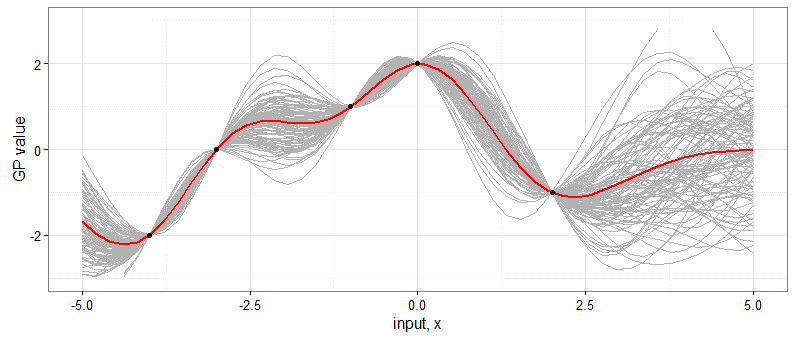
\includegraphics[width=0.95\linewidth]{../../gp_example}
\caption{Figure caption}
\label{gp_ex}
\end{figure}



GPs are advantageous for emulating computationally expensive deterministic computer code because 
\vspace{-15mm}
\begin{itemize}
\item Use of a GP does not require detailed foreknowledge of the approximate parametric form of the model; we often lack such knowledge
\item GPs easily interpolate the observed data; since the simulation code is deterministic and free of observation error, this is desirable
\item The variance of GPs provides a natural form of uncertainty quantification (see Figure \ref{gp_ex})
\end{itemize}



\end{block}


%----------------------------------------------------------------------------------------

\end{column} % End of column 2.1

\begin{column}{\onecolwid}\vspace{-.6in} % The second column within column 2 (column 2.2)

%----------------------------------------------------------------------------------------
%	METHODS
%----------------------------------------------------------------------------------------

\begin{block}{Emulator implementation}

Our model inputs are a dummy input $x_1$ (to convert our trivariate output into univariate), temperature $x_2$, volume fraction $x_3$ and thickness $x_4$. For our GP emulator prior we use the covariance function
\[
V(\mathbf x,\mathbf x' ) = \frac1\lambda \exp\{-\sum_{i=1}^4 \beta_i(x_i-x_i')^2 \}
\]
where $\lambda,\boldsymbol \beta$ were estimated using gradient methods to find their MLEs. 
% Ref, + more expl?
A prior mean $\mu(\mathbf x) = 0$ was also used. Observations $\eta(\mathbf x_i)$, $i=1,\cdots,504$ were collected from the simulation model using a LHC design. %ref?
The updated (posterior) GP emulator has mean given by
\[\mu^*(\mathbf x) = v(\mathbf x)^T \Sigma^{-1} \boldsymbol \eta \]
where $v(\mathbf x) = (V(\mathbf x, \mathbf x_1),\cdots,V(\mathbf x,\mathbf x_{504}))^T$, $\Sigma$ is a matrix with $\Sigma_{i,j} = V(\mathbf x_i,\mathbf x_j)$, and $\boldsymbol \eta = (\eta(\mathbf x_1),\cdots,\eta(\mathbf x_{504}))^T$. The updated covariance is 
\[
V^* (\mathbf x, \mathbf x') = V(\mathbf x, \mathbf x') - v(\mathbf x)^T \Sigma^{-1} v(\mathbf x')
\]
\end{block}

%----------------------------------------------------------------------------------------

\begin{block}{Desired data}

We calibrate the model to ``desired data'' which reflect extremely low tip deflection, rotation, and cost. Because we are antecedently ignorant of how close the model can come to our desired data, we place an improper $1/\sigma^2$ prior on the observation variance of each model output. We considered a range of desired outcomes.

\end{block}

\end{column} % End of column 2.2

\end{columns} % End of the split of column 2 - any content after this will now take up 2 columns width

%----------------------------------------------------------------------------------------
%	IMPORTANT RESULT
%----------------------------------------------------------------------------------------

\begin{alertblock}{Central idea}

Previous explorations of computer model calibration have approached calibration as a matter of bringing a computer model into agreement with physical reality. \textbf{In the present work, we consider computer model calibration as a method for design.} Under this framework, we calibrate a computer model not using physical experimental data, but rather using ``desired data'' which describes the performance one hopes to achieve in the simulated system. 

\end{alertblock} 

%----------------------------------------------------------------------------------------

\begin{columns}[t,totalwidth=\twocolwid] % Split up the two columns wide column again

\begin{column}{\onecolwid} % The first column within column 2 (column 2.1)

%----------------------------------------------------------------------------------------
%	MATHEMATICAL SECTION
%----------------------------------------------------------------------------------------

\begin{block}{Mathematical Section}

Nam quis odio enim, in molestie libero. Vivamus cursus mi at nulla elementum sollicitudin. Nam quis odio enim, in molestie libero. Vivamus cursus mi at nulla elementum sollicitudin.
  
\begin{equation}
E = mc^{2}
\label{eqn:Einstein}
\end{equation}

Nam quis odio enim, in molestie libero. Vivamus cursus mi at nulla elementum sollicitudin. Nam quis odio enim, in molestie libero. Vivamus cursus mi at nulla elementum sollicitudin.

\begin{equation}
\cos^3 \theta =\frac{1}{4}\cos\theta+\frac{3}{4}\cos 3\theta
\label{eq:refname}
\end{equation}

Nam quis odio enim, in molestie libero. Vivamus cursus mi at nulla elementum sollicitudin. Nam quis odio enim, in molestie libero. Vivamus cursus mi at nulla elementum sollicitudin.

\begin{equation}
\kappa =\frac{\xi}{E_{\mathrm{max}}} %\mathbb{ZNR}
\end{equation}

\end{block}

%----------------------------------------------------------------------------------------

\end{column} % End of column 2.1

\begin{column}{\onecolwid} % The second column within column 2 (column 2.2)

%----------------------------------------------------------------------------------------
%	RESULTS
%----------------------------------------------------------------------------------------

\begin{block}{Results}

\begin{figure}

\includegraphics[width=0.8\linewidth]{placeholder.jpg}
\caption{Figure caption}
\end{figure}

Nunc tempus venenatis facilisis. Curabitur suscipit consequat eros non porttitor. Sed a massa dolor, id ornare enim:

\begin{table}
\vspace{2ex}
\begin{tabular}{l l l}
\toprule
\textbf{Treatments} & \textbf{Response 1} & \textbf{Response 2}\\
\midrule
Treatment 1 & 0.0003262 & 0.562 \\
Treatment 2 & 0.0015681 & 0.910 \\
Treatment 3 & 0.0009271 & 0.296 \\
\bottomrule
\end{tabular}
\caption{Table caption}
\end{table}

\end{block}

%----------------------------------------------------------------------------------------

\end{column} % End of column 2.2

\end{columns} % End of the split of column 2

\end{column} % End of the second column

\begin{column}{\sepwid}\end{column} % Empty spacer column

\begin{column}{\onecolwid} % The third column

%----------------------------------------------------------------------------------------
%	CONCLUSION
%----------------------------------------------------------------------------------------

\begin{block}{MCMC implementation}

\begin{itemize}

\item Calibrate volume fraction and thickness to the desired data. Set a uniform prior over each.

\item Each iteration of the MCMC, draw new values for volume fraction, thickness, and the observation variances for each of tip deflection, rotation, and cost $(\sigma^2_{d},\sigma^2_{r},\sigma^2_{c}$). 

\item Where $\mathbf y$ is the desired data, $\mathcal D = (\mathbf y,\boldsymbol \eta)^T$ and $\Sigma_{\mathcal D} = \mathrm {Var}(\mathcal D)$, the likelihood of $\mathcal D$ is
\[%\begin{multline*}
L(\mathcal D| x_3,x_4,\lambda,\boldsymbol \beta,\Sigma_{\mathcal D}) = 
|\Sigma_{\mathcal D} | ^{-\frac 12} \exp \{ -\frac 12 \mathcal D ^T \Sigma_{\mathcal D}^{-1} \mathcal D  \}
\]%\end{multline*}
hence the full posterior density is
\begin{flalign*}
\pi(x_3,x_4,\sigma^2_d,\sigma^2_r,\sigma^2_c) \propto &&
\end{flalign*}

\vspace{-20mm}
\begin{eqnarray*}
\phantom = &L(\mathcal D| x_3,x_4,\lambda,\boldsymbol \beta,\Sigma_{\mathcal D}) \times &
\pi(x_3)\times \pi(x_4) \times \\&& \pi(\sigma^2_d) \times \pi (\sigma^2_r) \times \pi(\sigma^2_c)\\
=&L(\mathcal D| x_3,x_4,\lambda,\boldsymbol \beta,\Sigma_{\mathcal D}) \times& \frac1{\sigma^2_d\sigma^2_r\sigma^2_c}
\end{eqnarray*}


\item We eliminate boundary constraints with $z_i = \mathrm{logit}(x_i)$, $\tau_j = \log(\sigma^2_j)$ for $i=3,4$, $j=d,r,c$.

\item Metropolis-Hastings %ref
algorithm is used with normal proposals on $z_i^{(n)}|z_i^{(n-1)}$ and $\tau_j^{(n)}|\tau_j^{(n-1)}$, $\forall i \forall j$.

\end{itemize}



\end{block}

%----------------------------------------------------------------------------------------
%	ADDITIONAL INFORMATION
%----------------------------------------------------------------------------------------

\begin{block}{Additional Information}

Maecenas ultricies feugiat velit non mattis. Fusce tempus arcu id ligula varius dictum. 
\begin{itemize}
\item Curabitur pellentesque dignissim
\item Eu facilisis est tempus quis
\item Duis porta consequat lorem
\end{itemize}

\end{block}

%----------------------------------------------------------------------------------------
%	REFERENCES
%----------------------------------------------------------------------------------------

\begin{block}{References}

\nocite{*} % Insert publications even if they are not cited in the poster
\small{\bibliographystyle{unsrt}
\bibliography{sample}\vspace{0.75in}}

\end{block}

%----------------------------------------------------------------------------------------
%	ACKNOWLEDGEMENTS
%----------------------------------------------------------------------------------------

\setbeamercolor{block title}{fg=red,bg=white} % Change the block title color

\begin{block}{Acknowledgements}

\small{\rmfamily{Nam mollis tristique neque eu luctus. Suspendisse rutrum congue nisi sed convallis. Aenean id neque dolor. Pellentesque habitant morbi tristique senectus et netus et malesuada fames ac turpis egestas.}} \\

\end{block}

%----------------------------------------------------------------------------------------
%	CONTACT INFORMATION
%----------------------------------------------------------------------------------------

\setbeamercolor{block alerted title}{fg=black,bg=norange} % Change the alert block title colors
\setbeamercolor{block alerted body}{fg=black,bg=white} % Change the alert block body colors

\begin{alertblock}{Contact Information}

\begin{itemize}
\item Web: \href{http://www.university.edu/smithlab}{http://www.university.edu/smithlab}
\item Email: \href{mailto:john@smith.com}{john@smith.com}
\item Phone: +1 (000) 111 1111
\end{itemize}

\end{alertblock}

\begin{center}
\begin{tabular}{ccc}

\includegraphics[width=0.4\linewidth]{logo.png} & \hfill & 
\includegraphics[width=0.4\linewidth]{logo.png}
\end{tabular}
\end{center}

%----------------------------------------------------------------------------------------

\end{column} % End of the third column

\end{columns} % End of all the columns in the poster

\end{frame} % End of the enclosing frame

\end{document}
